\documentclass{article}
\usepackage[utf8]{inputenc}
\usepackage{graphicx}
\usepackage{geometry}
\geometry{a4paper, margin=1in}
\usepackage{subcaption} 
\usepackage{float}

\title{CSCI 566 Assignment 2: Problem 2 Solution}
\author{}
\date{}

\begin{document}

\maketitle

\section*{1. Training Curves and Generated Images for the GAN}


\begin{figure}[H]
    \centering
    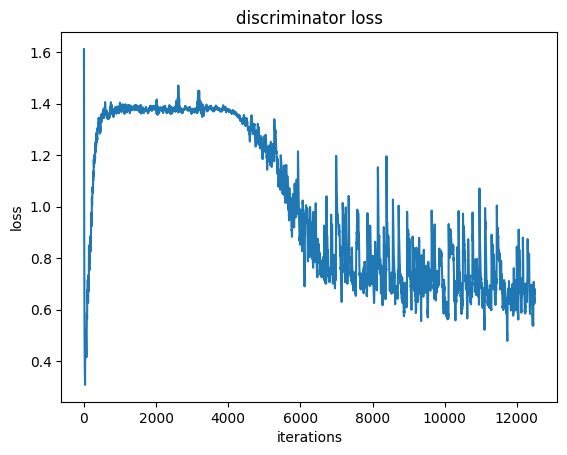
\includegraphics[width=0.8\textwidth]{gan_loss.png} 
    \caption{GAN Training Loss Curve}
\end{figure}


\begin{figure}[H]
    \centering
    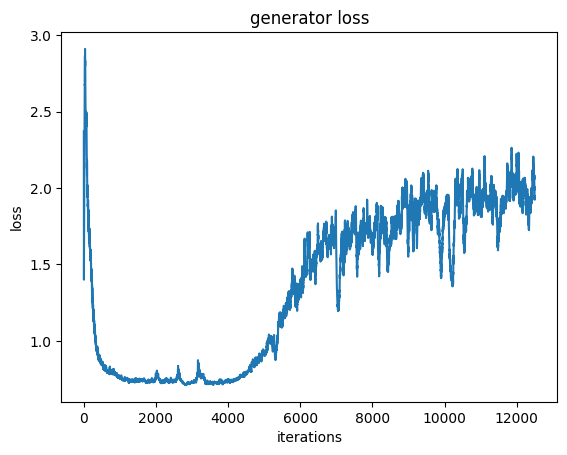
\includegraphics[width=0.8\textwidth]{gan_generated.png} 
    \caption{GAN Generated Images}
\end{figure}

\begin{figure}[H]
    \centering
    \begin{subfigure}{0.48\textwidth}
        \centering
        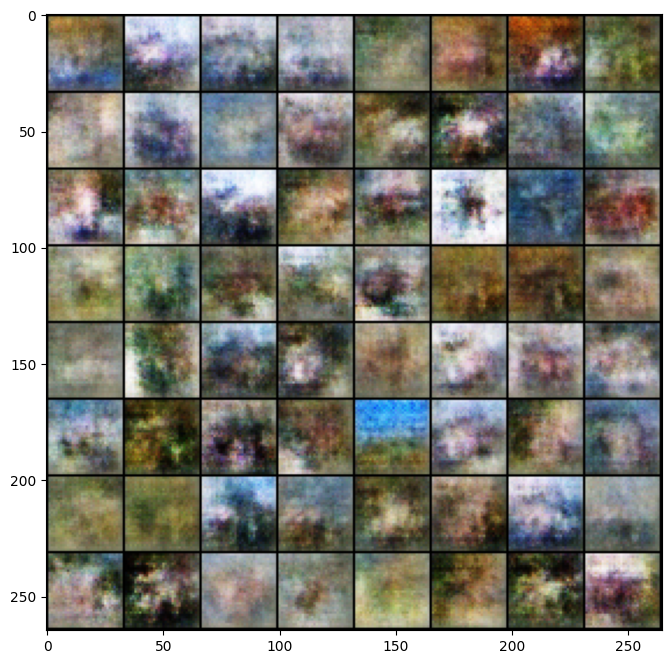
\includegraphics[width=\linewidth]{gan_recon.png}
        \caption{GAN Reconstruction Results}
    \end{subfigure}
    \hfill
    \begin{subfigure}{0.48\textwidth}
        \centering
        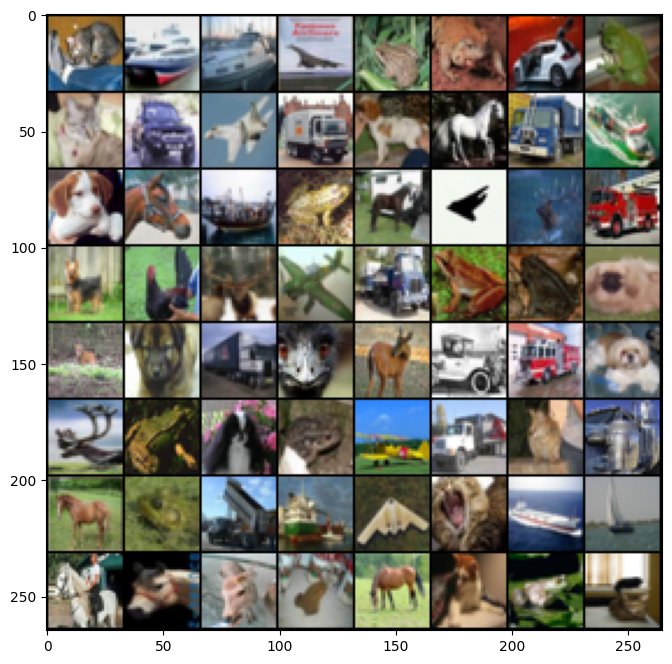
\includegraphics[width=\linewidth]{gan_samples.png}
        \caption{Samples}
    \end{subfigure}
    \caption{Reconstructions v.s. samples.}
\end{figure}


\section*{2. Answers to Inline Questions about GANs}

\textbf{Problem 2-2: The forger versus the police, revisited}

The primary flaw in the analogy is the assumption that the police (discriminator) is a "black box" to the forger (generator). In reality, the generator does not just look at the final classification output (e.g., "real" or "fake") and blindly guess how to improve. Instead, because neural networks are differentiable, the generator relies on the gradients flowing backward directly \textit{through} the discriminator. The discriminator acts as a differentiable mathematical function (a "white box" during the backward pass), allowing the generator to compute exactly how to adjust its weights to increase the probability of fooling the discriminator.

\vspace{1.5em}

\textbf{Problem 2-3: The Batch Normalization dilemma}

To solve this without omitting layers or changing their standard operational modes, we could concatenate the real and fake samples into a single, mixed batch for the discriminator's forward pass. To prevent the generator from failing due to mismatched normalization environments (the issue raised in the first question), we must ensure that when training the generator, its generated batch is also evaluated alongside a batch of real data, keeping the batch statistics consistent across both the discriminator and generator training phases.

\end{document}